\documentclass[../../../../../main.tex]{subfiles}
\begin{document}
\subsection{Create the Abstract Syntax Tree}
I first implemented the normal sequential function and later I will implement the multi-threaded approach. Again like the methods before it this is a static function, since it relates to the class not the object itself.
\begin{minted}[
frame=lines,
framesep=2mm,
linenos,
breaklines
]{java}
// create the abstract syntax tree for the expression - single-threaded
private static BinaryTree createTree(String expression) throws UnequalBracketsException {
	// remove enclosing matching brackets
	expression = checkBracket(expression);
	// find the least significant operator, if an operator remains
	int leastSigOperatorPos = leastSigOperatorPos(expression);
	if (leastSigOperatorPos == -1) { // base case - no operators remain
		return new BinaryTree(expression);
	} else { // recursive case - recurse on the sub-expressions
		// locate and hold the operator
		String operator = String.valueOf(expression.charAt(leastSigOperatorPos));
		// split the expression into sub-expressions by the operator and recurse on them
		String a = expression.substring(0, leastSigOperatorPos);
		String b = expression.substring(leastSigOperatorPos + 1);
		// return the new tree containing the trees of the sub-expressions and the
		// operator as the root value
		return new BinaryTree(operator, createTree(a), createTree(b));
	}
}
\end{minted}
The problem with creating a tree is that I can't actually display it in a way to check if my algorithm works. To get around this issue I can just use my traversal algorithm. I have tested my traversal algorithm and know that it works hence I can just output the stack from traversing it. I will standardize my expressions before I create the trees since this is what will happen in the constructor later.
\begin{minted}[breaklines]{java}
//  create the standardized expressions
String a = standardize("2^x");
String b = standardize("(x+1)(x-1)");
// create the trees
BinaryTree treeA = createTree(a);
BinaryTree treeB = createTree(b);
// show the conversion between the expressions and trees
// the traverse function uses a stack so remember the output will be reversed
// [2, x, ^] but it will be reversed therefore [^, x, 2]
System.out.println(a + " -> " + treeA.traverse());
// [x, 1, +, x, 1, -, *] but it will be reversed therefore [*, -, 1, x, +, 1, x]
System.out.println(b + " -> " + treeB.traverse());
\end{minted}
Here are the results:
\begin{minted}[breaklines]{console}
2^x -> [^], x, 2
(x+1)*(x-1) -> [*], -, 1, x, +, 1, x
\end{minted}
Which is exactly what I expected.
\newpage \noindent
When I designed this algorithm I wrote about how I could implement it using multiple threads. While multi-threading can be very powerful, like everything in Computer Science there is a cost. This is especially true where in \texttt{Java} the cost of instantiating a thread\cite{threadCreationJava} (on the fly at least) is incredibly expensive. In the article it talks about three main things:
\begin{enumerate}
\item Allocating Memory to the thread
\item Create the call stack for the thread\cite{threadStackJava, callStack}
\item Initialize and link the thread to the host OS
\end{enumerate}
This takes a lot of processing time, in this article\cite{threadCreationRate} one user manages to spawn about 10000 threads a second, which means that it takes approximately $0.1$ seconds to spawn every thread. This is to be taken with a pinch of salt however since the article is quite old (8 years in fact) and processors are better and the JVM should be more efficient nowadays than before. To test this for myself I ran their benchmark program.
\footnote{The code for this is on the StackOverflow thread, made by a user called, at the time of writing this, ``Jaan''\cite{threadCreationRate}} 
I did change some of the parameters to make each test do the same amount of work (the same number of instructions) and made the number of threads spawned different as well. I also ran it 3 times so I could calculate a mean to able to identify anomalous data. This also alleviates some of the randomness of the schedulerI did this by compiling and executing the program 3 times, to reduce the effect of cached memory affecting the results. While the test does accommodate for this issue and allows for multiple tests, I think it is best to give the JVM no chance for optimization by just destroying and recreating the JVM. The results table and the corresponding graphs are on the next page.
\[DO \cdot THE \cdot THREAD \cdot CREATION \cdot TEST\]
\[do \cdot the \cdot analysis\]
\begin{landscape}
\begin{table}[ht]
\centering
\caption{Thread Creation Test}
 \setlength{\tabcolsep}{0.2em}
\sisetup{tight-spacing=true}
\begin{tabular}{| l | S[table-format=4.2] | S[table-format=4.2] | S[table-format=4.2] | S[table-format=4.2] | S[table-format=4.2] | S[table-format=4.2] | S[table-format=4.2] | S[table-format=4.2] | S[table-format=4.2] | S[table-format=4.2] | S[table-format=4.2] | S[table-format=4.2] | S[table-format=4.2] |}
\hline
\multicolumn{1}{|c|}{\multirow{3}{*}{\parbox{1.65cm}{Number of Threads}}} & \multicolumn{13}{c|}{Time Taken/\si{\milli\second}}                                                                                                                                                                                                                                                                                                              \\ \cline{2-14} 
\multicolumn{1}{|c|}{}                                   & \multicolumn{4}{c|}{To Create}                                                                       & \multicolumn{4}{c|}{To Complete Work}                                                                & \multicolumn{4}{c|}{To Join}                                                                         &  \multicolumn{1}{c|}{\multirow{2}{*}{Mean Total}} \\ \cline{2-13}
\multicolumn{1}{|c|}{}                                   & \multicolumn{1}{c|}{1} & \multicolumn{1}{c|}{2} & \multicolumn{1}{c|}{3} & \multicolumn{1}{c|}{Mean} & \multicolumn{1}{c|}{1} & \multicolumn{1}{c|}{2} & \multicolumn{1}{c|}{3} & \multicolumn{1}{c|}{Mean} & \multicolumn{1}{c|}{1} & \multicolumn{1}{c|}{2} & \multicolumn{1}{c|}{3} & \multicolumn{1}{c|}{Mean} &                             \\ \hline
1 		&1.0 &1.0 &1.0 &1.0 &1.0 &1.0 &1.0 &1.0 &1.0 &1.0 &1.0 &1.0 & 1.0
\\ \hline
2 		&1.0 &1.0 &1.0 &1.0 &1.0 &1.0 &1.0 &1.0 &1.0 &1.0 &1.0 &1.0 & 1.0
\\ \hline
5 		&1.0 &1.0 &1.0 &1.0 &1.0 &1.0 &1.0 &1.0 &1.0 &1.0 &1.0 &1.0 & 1.0
\\ \hline
20 		&1.0 &1.0 &1.0 &1.0 &1.0 &1.0 &1.0 &1.0 &1.0 &1.0 &1.0 &1.0 & 1.0
\\ \hline
100 	&1.0 &1.0 &1.0 &1.0 &1.0 &1.0 &1.0 &1.0 &1.0 &1.0 &1.0 &1.0 & 1.0
\\ \hline
1000 	&1.0 &1.0 &1.0 &1.0 &1.0 &1.0 &1.0 &1.0 &1.0 &1.0 &1.0 &1.0 & 1.0
\\ \hline
\end{tabular}
\label{tbl:threadCreationTest}
\end{table}
\begin{figure}[H]
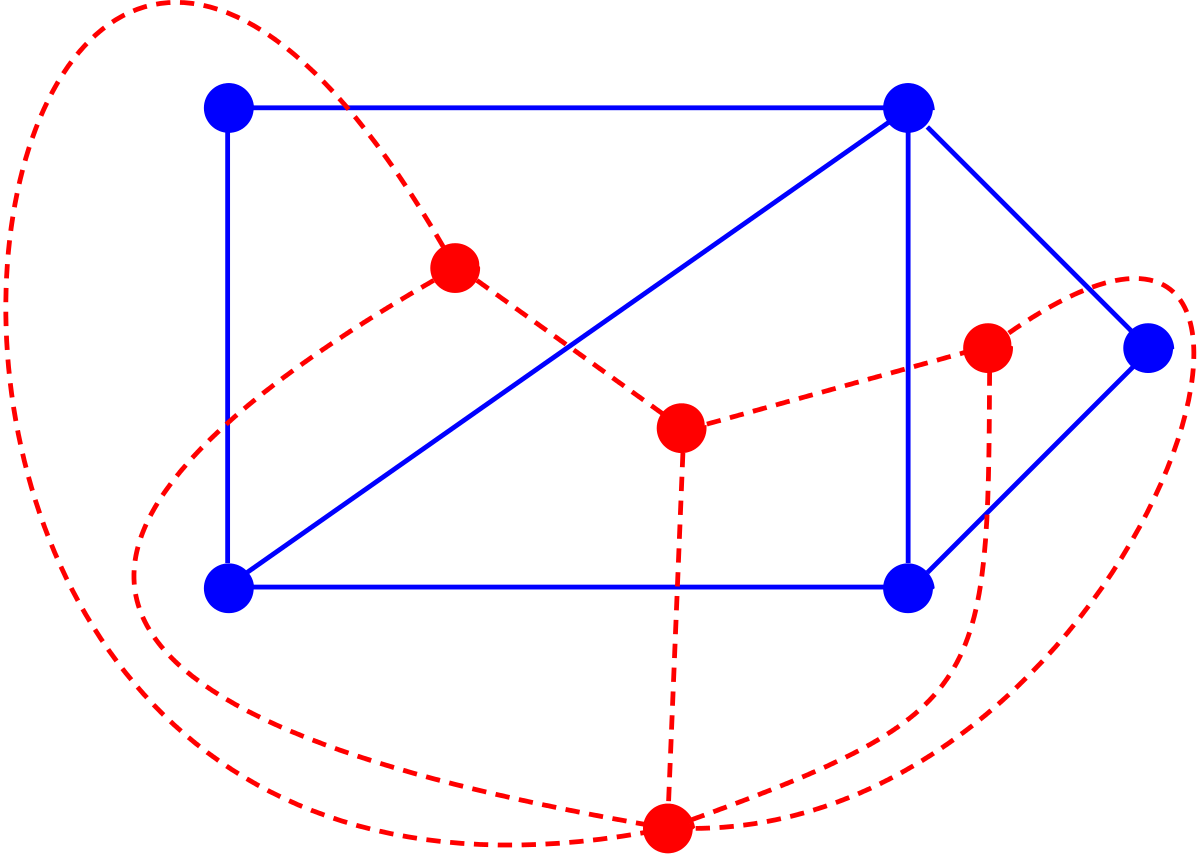
\includegraphics[height=0.25\textheight]{graphs/i.png}
\end{figure}
\end{landscape}
\noindent
From the analysis above it seems that the effect of using a few threads seems minimal and the overhead may be outweighed by the performance gain from other parts of the function. However this may be specific to this scenario, so to test this properly I implemented the multi-threaded version which is below:
\begin{minted}[
frame=lines,
framesep=2mm,
linenos,
breaklines
]{java}
// create the abstract syntax tree for the expression - multi-threaded
private static BinaryTree createTreeThread(String expression)
		throws StringIndexOutOfBoundsException, UnequalBracketsException, InterruptedException, ExecutionException {
	// remove enclosing matching brackets
	expression = checkBracket(expression);
	// find the least significant operator, if an operator remains
	int leastSigOperatorPos = leastSigOperatorPos(expression);
	if (leastSigOperatorPos == -1) { // base case - no operators remain
		return new BinaryTree(expression);
	} else { // recursive case - recurse on the sub-expressions
		// locate and hold the operator
		String operator = String.valueOf(expression.charAt(leastSigOperatorPos));
		// split the expression into sub-expressions by the operator and recurse on them
		String a = expression.substring(0, leastSigOperatorPos);
		String b = expression.substring(leastSigOperatorPos + 1);
		BinaryTree tree0;
		BinaryTree tree1;
		// create the threads and execute them
		ExecutorService executor0 = Executors.newSingleThreadExecutor();
		Future<BinaryTree> future0 = executor0.submit(() -> {
			return createTree(a);
		});
		ExecutorService executor1 = Executors.newSingleThreadExecutor();
		Future<BinaryTree> future1 = executor1.submit(() -> {
			return createTree(b);
		});
		// return the tree values from the threads
		tree0 = future0.get();
		tree1 = future1.get();
		// shutdown the threads
		executor0.shutdown();
		executor1.shutdown();
		// return the new tree containing the trees of the sub-expressions and the
		// operator as the root value
		return new BinaryTree(operator, tree0, tree1);
	}
}
\end{minted}
\newpage\noindent
I then tried to test my 2 \texttt{createTree()} functions to identify if a purely single-threaded approach is more efficient than a multi-threaded approach. However the two approaches may change in effectiveness depending on the complexity of the expression we are parsing. In order to control this for a fair test we need to effectively measure the complexity hence we need to analyze the algorithm in detail.

Assuming that a single call of the \texttt{createTree()} algorithm takes the same time, $t$, to execute (exclude the recursive calls and the overhead that is need for them), then $\mathcal{O}(n) = n+1$ where $n$ is the number of operators. Assuming that the expression is valid, this value comes from the fact that we can split a standardized expression into by each operator. From the nature of our approach, there will be no operators on the start or the end of a valid expression, and each variable/constant is split apart by an operator\footnote{This is an inherent property within any valid expression since otherwise without this we cannot separate each variable/constant hence we cannot define explicitly where each variable/constant starts and ends. Within human expressions this is more implicit but still exists. For example $(x+1)(y-1)$ appears not to have an operator between 1 and $y$, but recall from the design section that this expression actual means $(x+1)*(y-1)$ hence the property is still valid. We have only applied this to operators and becomes blurred when we talk about functions within our expression, such as $\sin$, but this does not matter since our algorithm does not deal with this.}. 
Now from this property we notice that each operator has a uniquely positioned variable/constant on the right of it, apart from the first operator which has an extra variable/constant to the left of it. Now our function recurses $k$ times where k is the number of base sub-expressions, i.e.\ variables/constants. However it can be hard to count these variables/constants since they can be of variable length (1.2 is a constant and has a length in terms of strings of 3, but $x$ is also a variable but has a length of 1). On the other hand operators are incredibly easy to spot and count since there is a finite number of types of operators, and they are all of length 1. Hence it makes sense to define the complexity of our function in terms of the number of operators. This means that one of our independent variables, the one we will change, will be the number of operators. We will also change whether we use threads or not since this is the point of our experiment.
 
\begin{table}[ht]
\caption{Single- vs Multi-Threaded Approach Test}
\centering
\sisetup{tight-spacing=true}
\begin{tabular}{| l | S[table-format=3.2] | S[table-format=3.2] | S[table-format=3.2] | S[table-format=3.2] | S[table-format=3.2] | S[table-format=3.2] | S[table-format=3.2] | S[table-format=3.2] |}
\hline
\multicolumn{1}{|c|}{\multirow{3}{*}{\parbox{1.65cm}{Number of Operators}}} & \multicolumn{8}{c|}{Time Taken/\si{\milli\second}}                                                                                                                                                                          \\ \cline{2-9} 
\multicolumn{1}{|c|}{}                                     & \multicolumn{4}{c|}{With Threads}                                                                    & \multicolumn{4}{c|}{Without Threads}                                                                 \\ \cline{2-9} 
\multicolumn{1}{|c|}{}                                     & \multicolumn{1}{c|}{1} & \multicolumn{1}{c|}{2} & \multicolumn{1}{c|}{3} & \multicolumn{1}{c|}{Mean} & \multicolumn{1}{c|}{1} & \multicolumn{1}{c|}{2} & \multicolumn{1}{c|}{3} & \multicolumn{1}{c|}{Mean} \\ \hline
1 		& insert & insert & insert & insert & insert & insert & insert & insert
\\ \hline
5 		& insert & insert & insert & insert & insert & insert & insert & insert
\\ \hline
20 		& insert & insert & insert & insert & insert & insert & insert & insert
\\ \hline
100 	& insert & insert & insert & insert & insert & insert & insert & insert
\\ \hline
\end{tabular}
\label{tbl:parseAlgorithmTest}
\end{table}



\newpage
\end{document}